\documentclass{article}
\usepackage{graphicx}
\usepackage[english]{babel}
\setlength{\paperwidth}{210mm}
\setlength{\paperheight}{160mm}
\usepackage[margin=0.5in]{geometry}
\usepackage{array}
\usepackage[utf8]{inputenc}
\usepackage{hyperref}
\usepackage{color}

\title{\colorbox{yellow}{CS 251 Project Report}}
\author{Sahil,Rajesh,Maniteja}
\begin{document}
\maketitle
\hfill
\begin{table}[h]
	\begin{center}
	\resizebox{11cm}{!}{
	\begin{tabular}{|c|c|l|}
	\hline
	Group Name & Roll No. & Name \\
	\hline
	 & 140050030 & Sahil \\ \cline{2-3}
	Synergy & 140050073 & Rajesh \\ \cline{2-3}
	 & 140050079 & Maniteja \\
	\hline
	\end{tabular}
	}
	\end{center}
\end{table}
\begin{center}
\section*{}
\large{
              Project Supervisor:{\huge Prof.Sharat Chandran }           
}
\end{center}

\clearpage
\section*{\huge{PROJECT SUMMARY}}
\large{
Our cs251 project is a 2D rube Goldberg machine implemented on the Box2D physics simulator.\\
 It is the simulation of a series of processes which results in the event of ”firing a bullet from canon”.\\
It serves the purpose of a security system.\\
 The working of this machine depends on the synchronous working of the following separate components (as given in the figure) .\\
\\
\\
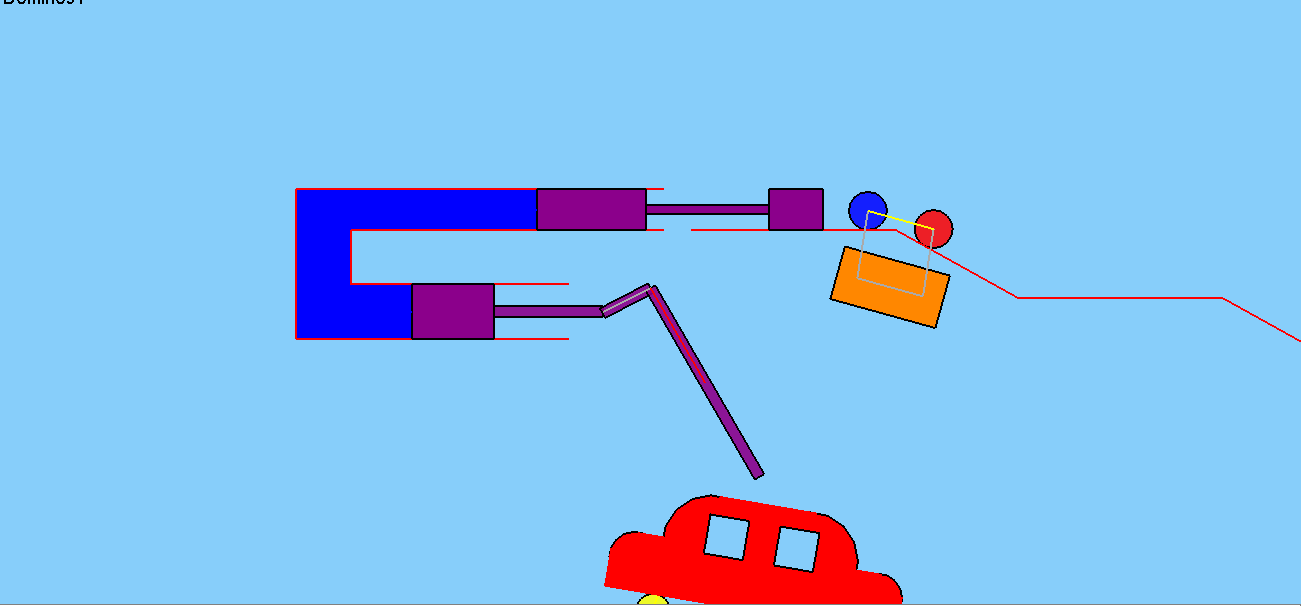
\includegraphics[width=0.8\textwidth, height=80mm]{1.png}
}
\section*{\huge{ DETAILED WORKING OF THE SIMULATION}}
\large{
The series of steps followed are shown below.
\\
\\
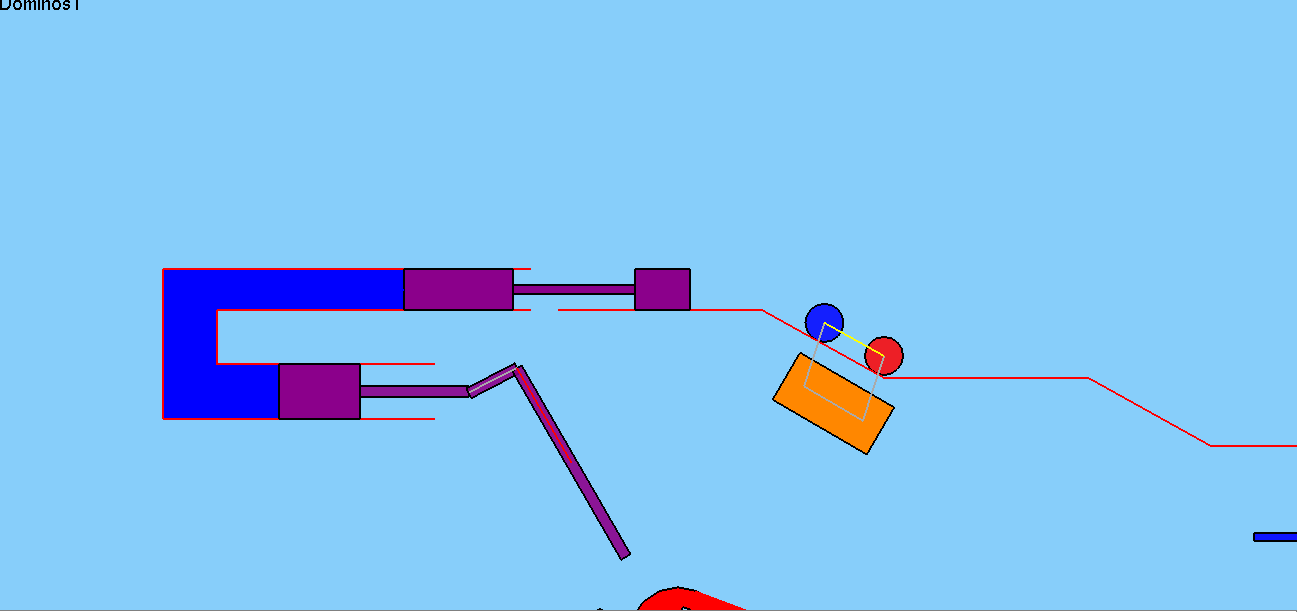
\includegraphics[width=0.8\textwidth, height=80mm]{2.png}
\\
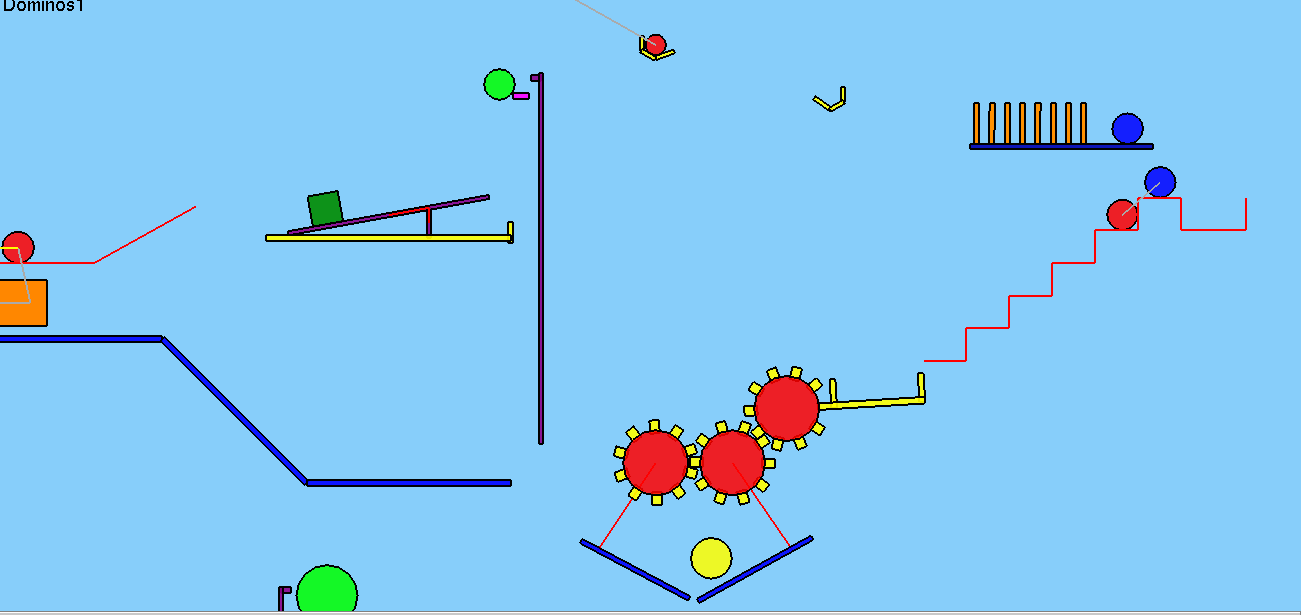
\includegraphics[width=0.8\textwidth, height=80mm]{3.png}
\\
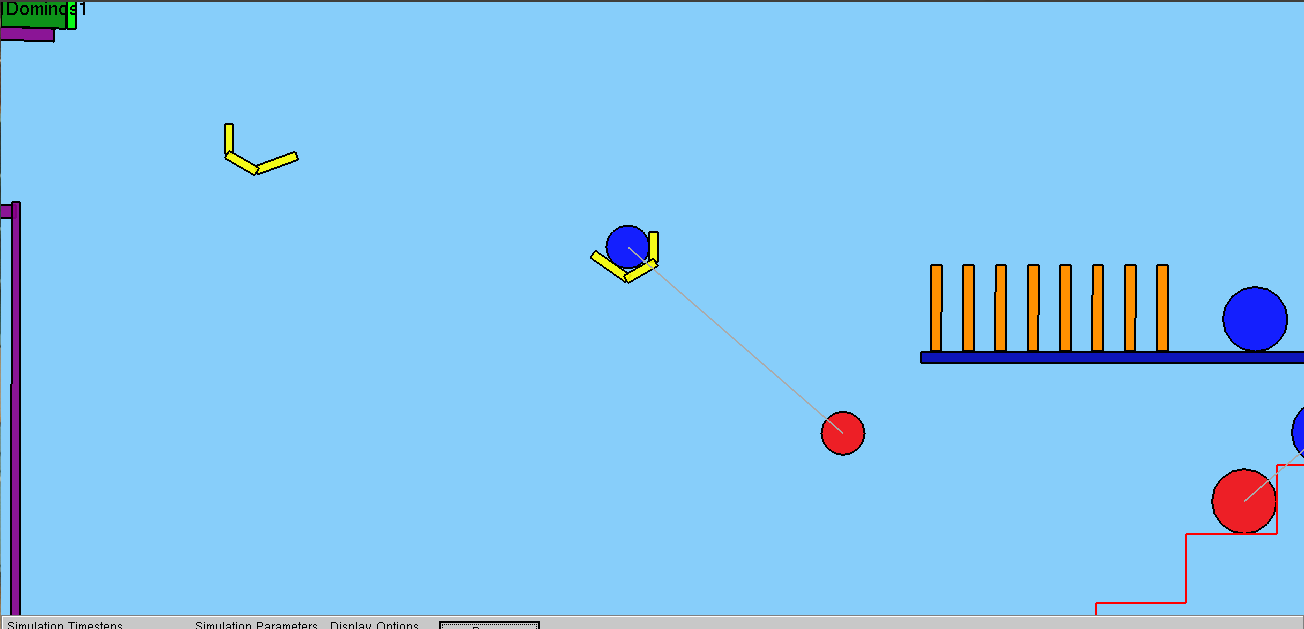
\includegraphics[width=0.8\textwidth, height=80mm]{4.png}
\\
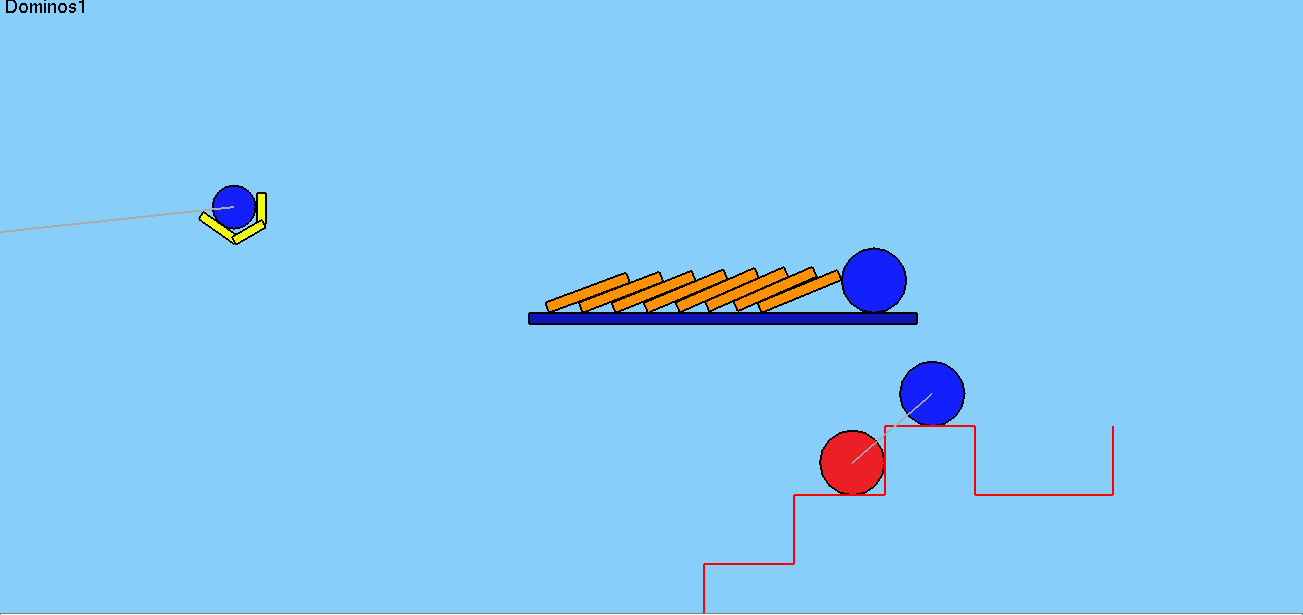
\includegraphics[width=0.8\textwidth, height=80mm]{5.png}
\\
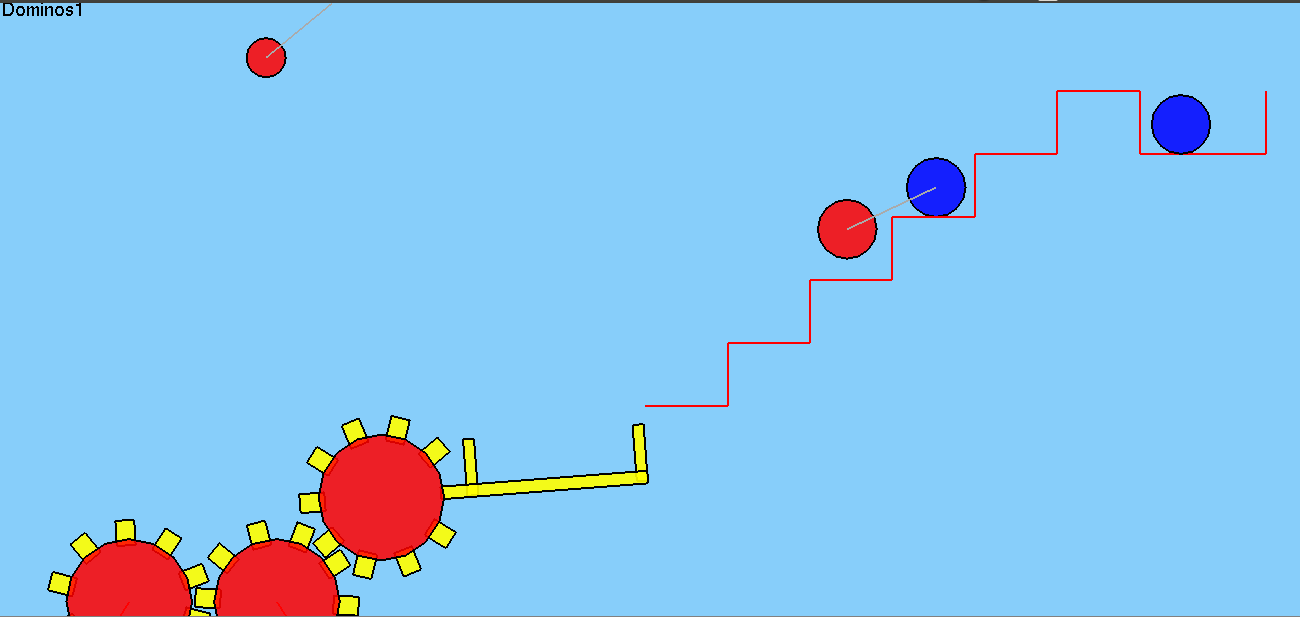
\includegraphics[width=0.8\textwidth, height=80mm]{6.png}
\\
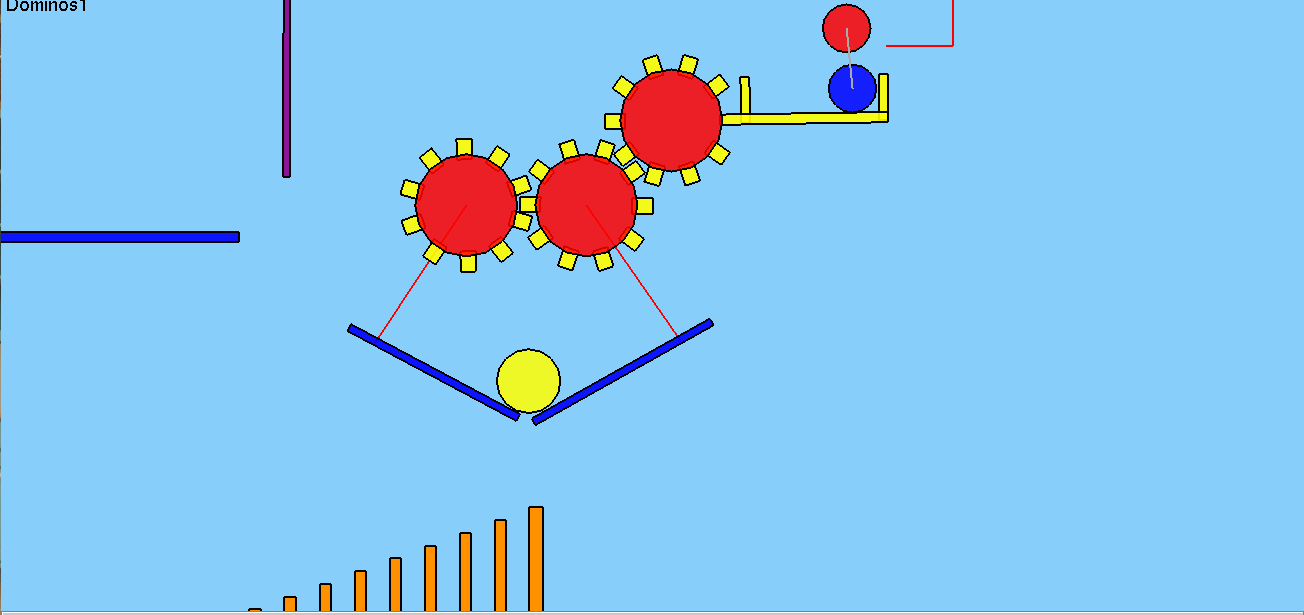
\includegraphics[width=0.8\textwidth, height=80mm]{7.png}
\\
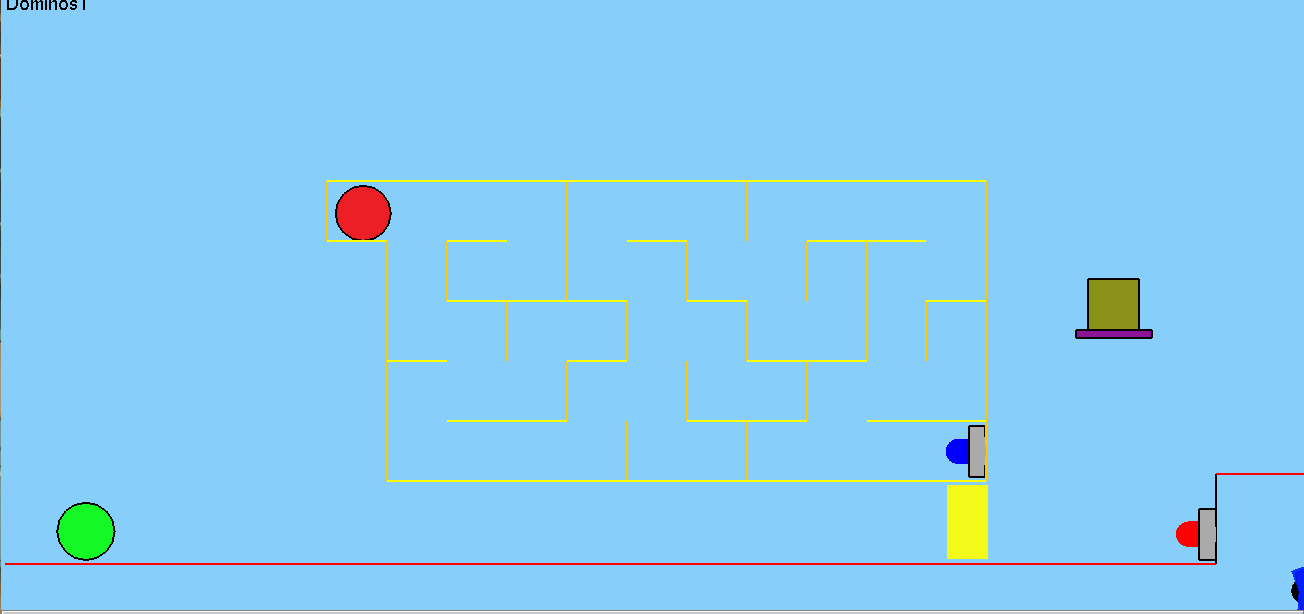
\includegraphics[width=0.8\textwidth, height=80mm]{8.png}
}
\clearpage
\section*{\huge{REAL LIFE PROJECT}}
\large{
We did this project as a part of the assignment , But we had a real experience on how a project is done.\\
We learnt  the following as a part of the project: \\
\\
{\huge Non Technical:}\\
\\
1.Team Work\\
2.Better Efficiency in doing large projects\\
3.Project management\\
4.Facing difficulties  and how we had to change our Project Proposal accordingly\\
\\
\\
{\huge Technical:}\\
\\
1.Using Box2d \\
2.Makefiles and all shell commands \\
3.Documentation using Doxygen\\
4.Presentation in Beamer and Bibtex\\
}
\clearpage
\section*{\huge{USE OF OUR BOX2D SIMULATOR IN REAL LIFE}}
\large{
Box2D is mainly used in games to make objects move in realistic ways and make the game world more interactive.\\
In our project the main idea is to stop the car from entering a zone using a security key ( In this case it is just a maze ) using only
mechanical elements and arranging them in a way to get the required.\\
The elements we used are very innovative ( not the usual kind ) and thus proposes a creative way of designing the Rube Goldberg Machines \\
Thus Box 2D is very helpful in simulating real physics problems and modelling them.\\
}
\clearpage
\section*{}
\hfill
\begin{thebibliography}{7}

\bibitem{einstein} 
\href{''http://box2d.org/''}{Box2D Website}

\bibitem{einstein} 
\href{''https://www.youtube.com/watch?v=0kqIChxrw-4''}{https://www.youtube.com/watch?v=0kqIChxrw4}

\bibitem{einstein} 
\href{''https://www.youtube.com/watch?v=bBIXpu-D_Zo''}{https://www.youtube.com/watch?v=bBIXpuDZo}

\bibitem{einstein} 
\href{''https://www.youtube.com/results?search_query=box2d''}{https://www.youtube.com/results?searchquery=box2d}
 
\bibitem{einstein} 
\href{''https://www.youtube.com/watch?v=8kZRpouZ3OQ''}{https://www.youtube.com/watch?v=8kZRpouZ3OQ}

\bibitem{einstein} 
\href{''https://www.youtube.com/watch?v=9fCT-EjlF9I''}{https://www.youtube.com/watch?v=9fCTEjlF9I}

\end{thebibliography}
\clearpage


\end{document}

